\documentclass[openary, a4paper, oneside]{jsarticle}

\input{../mymacro.tex}

\newcommand{\Dt}{\frac{d}{dt}}
\newcommand{\Ds}{\frac{d}{ds}}
\newcommand{\dt}{\partial_t}
\newcommand{\ds}{\partial_s}
\newcommand{\dnu}{\partial_{\nu}}

\newcommand{\sG}{_{\Gamma}}
\newcommand{\sS}{_{\Sigma}}

\newcommand{\veps}{\varepsilon}

\newcommand{\INTt}{\int_0^t}
\newcommand{\INTT}{\int_0^T}
\newcommand{\INTO}{\int_{\Omega}}
\newcommand{\INTG}{\int_{\Gamma}}

\newcommand{\weakto}{\rightharpoonup}
\newcommand{\weakstarto}{\overset{*}{\rightharpoonup}}
\newcommand{\emb}{\hookrightarrow}
\newcommand{\emp}{\hookleftarrow}

\newcommand{\Otani}{\^Otani}
\newcommand{\Holder}{H\"older}
\newcommand{\Schrodinger}{Schr\"odinger}
\newcommand{\Arzela}{Arzel\`a}
\newcommand{\Poincare}{Poincar\'e}
\newcommand{\Komura}{K\=omura}

\usepackage{tikz}
\usetikzlibrary{positioning}

\author{香川 渓一郎}
\date{\today}
\title{Cahn--Hilliard equation 関連論文}
\hypersetup{
	pdfkeywords={},
	pdfsubject={},
	pdfcreator={}
}

\renewcommand{\labelenumi}{(\arabic{enumi})}

\begin{document}

\maketitle
\tableofcontents

\newpage

\section{Kosugi, Morita, Yotsutani (2007) day:2020.03.12}
	\subsection{論文情報}
		Kosugi, Satoshi, Yoshihisa Morita, and Shoji Yotsutani. "Stationary solutions to the one-dimensional Cahn-Hilliard equation: proof by the complete elliptic integrals." Discrete and Continuous Dynamical Systems 19.4 (2007): 609.

	\subsection{何に関する論文で何を示したのか}
		空間1次元のカーン=ヒリアード方程式の定常解を書き下した.
		また拡散係数が消失する漸近極限でも大域分岐ダイアグラムを描いた.
		\begin{equation}\left\{\begin{array}{ll}
			\varepsilon^{2} \frac{d^{2} u}{d x^{2}}(x)+f(u(x))-a=0,\quad x \in(0,1) \\
			\frac{d u}{d x}(x)=0,\quad x=0,1 \\
			m=\int_{0}^{1} u(x) d x,\quad a=\int_{0}^{1} f(u(x)) d x
		\end{array} \right.\end{equation}
		但し$f(u) = u^3 - u$.

	\subsection{先行研究と比べてスゴイこと}
		解をヤコビの楕円関数と完全楕円積分を用いて陽に書き下した.

	\subsection{論文の核となるモノ}

	\subsection{どのような手法で示したのか}

	\subsection{今後の展望や課題}

	\subsection{この論文を引用している論文}
		\begin{itemize}
			\item Wakasa, Tohru, and Shoji Yotsutani. "Representation formulas for some 1-dimensional linearized eigenvalue problems." Communications on Pure and Applied Analysis 7.4 (2008): 745.
			\item Wakasa, Tohru, and Shoji Yotsutani. "Limiting classification on linearized eigenvalue problems for 1-dimensional Allen–Cahn equation I—asymptotic formulas of eigenvalues." Journal of Differential Equations 258.11 (2015): 3960-4006.
			\item Mori, Tatsuki, et al. "Exact multiplicity of stationary limiting problem of a cell polarization model." Discrete Contin. Dyn. Syst. Ser. A 36 (2016): 5627-5655.
			\item[$\star$] Miyamoto, Yasuhito. "Global bifurcation and stable two-phase separation for a phase field model in a disk." Discrete \& Continuous Dynamical Systems-A 30.3 (2011): 791.
			\item Tohru, Wakasa. "Note on parameter dependence of eigenvalues for a linearized eigenvalue problem." Pure Appl. Math 64 (2017): 1-12.
			\item Jimbo, Shuichi, and Yoshihisa Morita. "Nonlocal eigenvalue problems arising in a generalized phase-field-type system." Japan Journal of Industrial and Applied Mathematics 34.2 (2017): 555-584.
			\item 四ツ谷晶二. "数式処理の発想を利用した数学教育の試み (数学ソフトウェアと教育: 数学ソフトウェアの効果的利用に関する研究)." (2012).
			\item 森竜樹. "All Global Bifurcation Curves for a Cell Polarization Model (Theory of Biomathematics and Its Applications XII: Mathematical and experimental approach to clarify patterns in a transition process)." (2016).
		\end{itemize}

	\subsection{この論文が引用している主要な先行研究}

\newpage

\begin{thebibliography}{99}
	\bibitem{KosugiMoritaYotsutani2007}
	Kosugi, Satoshi, Yoshihisa Morita, and Shoji Yotsutani. "Stationary solutions to the one-dimensional Cahn-Hilliard equation: proof by the complete elliptic integrals." Discrete and Continuous Dynamical Systems 19.4 (2007): 609.
\end{thebibliography}

\appendix

\section{著者 (出版年) day:記録をつけた日}
	\subsection{論文情報}
		著者名, 論文タイトル, 掲載雑誌, 年, ページ.

	\subsection{何に関する論文で何を示したのか}

	\subsection{先行研究と比べてスゴイこと}

	\subsection{論文の核となるモノ}

	\subsection{どのような手法で示したのか}

	\subsection{今後の展望や課題}

	\subsection{この論文を引用している論文}

	\subsection{この論文が引用している主要な先行研究}

\newpage

%%%%%%%%%%%%%%%%%%%%%%%%%%%%%%%%%%%%%%%%%%%%%%%%%%%%%%%%
%%%%%%%%%%%%%%%%%%%%%%%%%%%%%%%%%%%%%%%%%%%%%%%%%%%%%%%%

\section{有向グラフのサンプル}
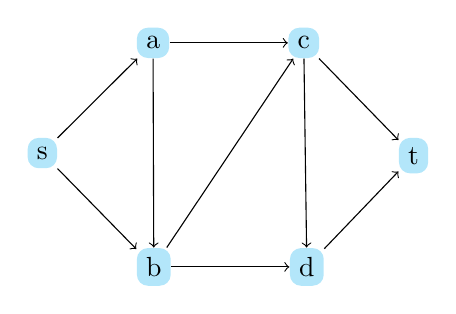
\begin{tikzpicture}[every node/.style={rectangle,fill=cyan!30,rounded corners}]
    \node (s) {s};
    \node[above right=of s] (a) {a};
    \node[below right=of s] (b) {b};
    \node[right=1.5cm of a] (c) {c};
    \node[right=1.5cm of b] (d) {d};
    \node[below right=of c] (t) {t};

    \foreach \u / \v in {s/a,s/b,a/b,a/c,b/c,b/d,c/d,c/t,d/t}
        \draw[->] (\u) -- (\v);
\end{tikzpicture}

\end{document}
